\chapter{传输层}

\section{多路复用与多路分解}

\subsection{传输层}

传输层协议为运行在不同主机上的应用进程之间提供了逻辑通信。在发送端,运输层将应用进程的报文添加传输层首部形成传输层分组,称为报文段(segment),这个过程被称为多路复用(multiplexing)。在接收端,网络层从数据报中提取传输层报文段,并交付给传输层,传输层处理报文段,将数据交付给应用进程,这个过程被称为多路分解(demultiplexing)。\\

应用层可以使用UDP和TCP这两种截然不同的传输层协议。其中UDP提供了一种不可靠、无连接的服务,因此,UDP不能保证一个进程发送的数据能够完整无缺地到达目的进程。而TCP提供了一种可靠的、面向连接的服务,通过使用流量控制、序号、确认和定时器,TCP确保正确地、按序地将数据交付给接收进程。\\

\subsection{无连接的多路复用/多路分解}

一个UDP的socket是由一个二元组进行标识的,该二元组包含了目的IP地址和目的端口号。如果两个UDP报文段来自不同的源IP地址或源端口号,但是具有相同的目的IP和目的端口号,那么这两个报文段将通过相同的socket被发送到相同的目的进程。\\

使用UDP时,当A给B发送的报文段中,源端口号是用作返回地址的一部分。当B回发一个报文段给A时,就需要从A到B的报文段中取值。\\

\begin{figure}[H]
	\centering
	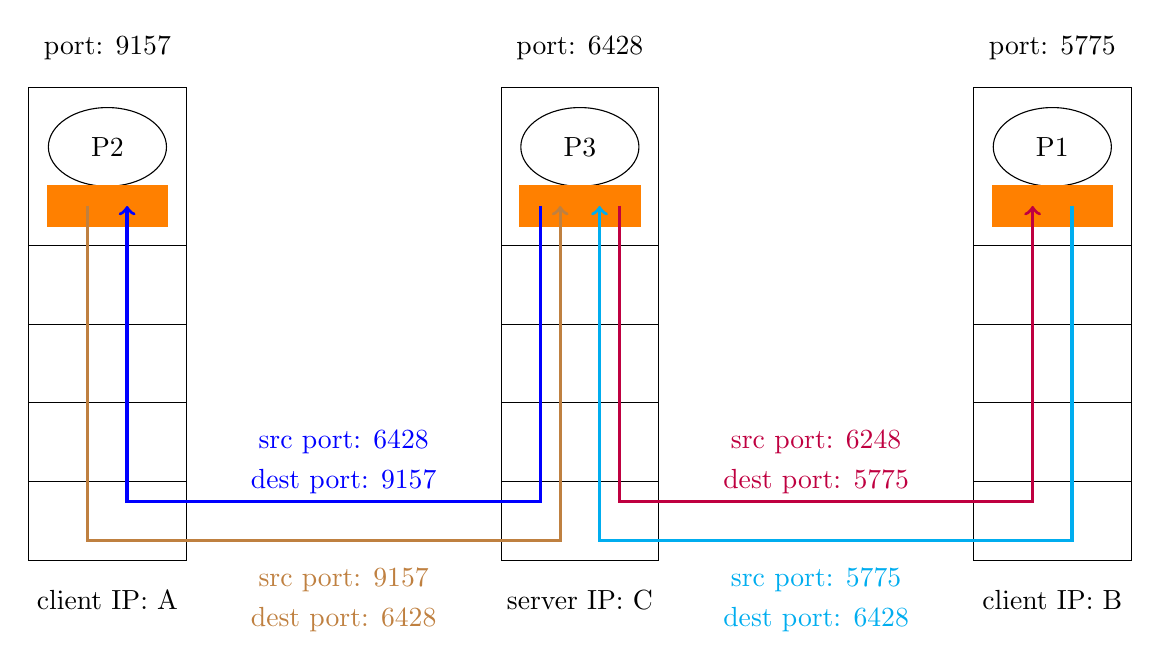
\begin{tikzpicture}
		\draw (1,6.5) node {port: 9157};
		\draw (0,0) rectangle (2,6);
		\draw (0,1) -- (2,1);
		\draw (0,2) -- (2,2);
		\draw (0,3) -- (2,3);
		\draw (0,4) -- (2,4);
		\draw (1,-0.5) node {client IP: A};
		\draw (1,5.25) ellipse (0.75 and 0.5);
		\draw (1,5.25) node {P2};
		\draw[orange, very thick, fill] (0.25,4.25) rectangle (1.75,4.75);

		\draw (7,6.5) node {port: 6428};
		\draw (6,0) rectangle (8,6);
		\draw (6,1) -- (8,1);
		\draw (6,2) -- (8,2);
		\draw (6,3) -- (8,3);
		\draw (6,4) -- (8,4);
		\draw (7,-0.5) node {server IP: C};
		\draw (7,5.25) ellipse (0.75 and 0.5);
		\draw (7,5.25) node {P3};
		\draw[orange, very thick, fill] (6.25,4.25) rectangle (7.75,4.75);

		\draw (13,6.5) node {port: 5775};
		\draw (12,0) rectangle (14,6);
		\draw (12,1) -- (14,1);
		\draw (12,2) -- (14,2);
		\draw (12,3) -- (14,3);
		\draw (12,4) -- (14,4);
		\draw (13,-0.5) node {client IP: B};
		\draw (13,5.25) ellipse (0.75 and 0.5);
		\draw (13,5.25) node {P1};
		\draw[orange, very thick, fill] (12.25,4.25) rectangle (13.75,4.75);

		\draw[->, very thick, brown] (0.75,4.5) -- (0.75,0.25) -- (6.75,0.25) -- (6.75,4.5);
		\draw[brown] (4,-0.25) node {src port: 9157};
		\draw[brown] (4,-0.75) node {dest port: 6428};

		\draw[->, very thick, blue] (6.5,4.5) -- (6.5,0.75) -- (1.25,0.75) -- (1.25,4.5);
		\draw[blue] (4,1.5) node {src port: 6428};
		\draw[blue] (4,1) node {dest port: 9157};

		\draw[->, very thick, cyan] (13.25,4.5) -- (13.25,0.25) -- (7.25,0.25) -- (7.25,4.5);
		\draw[cyan] (10,-0.25) node {src port: 5775};
		\draw[cyan] (10,-0.75) node {dest port: 6428};

		\draw[->, very thick, purple] (7.5,4.5) -- (7.5,0.75) -- (12.75,0.75) -- (12.75,4.5);
		\draw[purple] (10,1.5) node {src port: 6248};
		\draw[purple] (10,1) node {dest port: 5775};
	\end{tikzpicture}
	\caption{无连接的多路复用与多路分解}
\end{figure}

\vspace{0.5cm}

\subsection{面向连接的多路复用与多路分解}

TCP的socket是由一个四元组来标识的,其中包括了源IP地址、源端口号、目的IP地址和目的端口号。与UDP不同的是,两个具有不同源IP地址或源端口号的TCP报文段将被发送到两个不同的socket。\\

\begin{figure}[H]
	\centering
	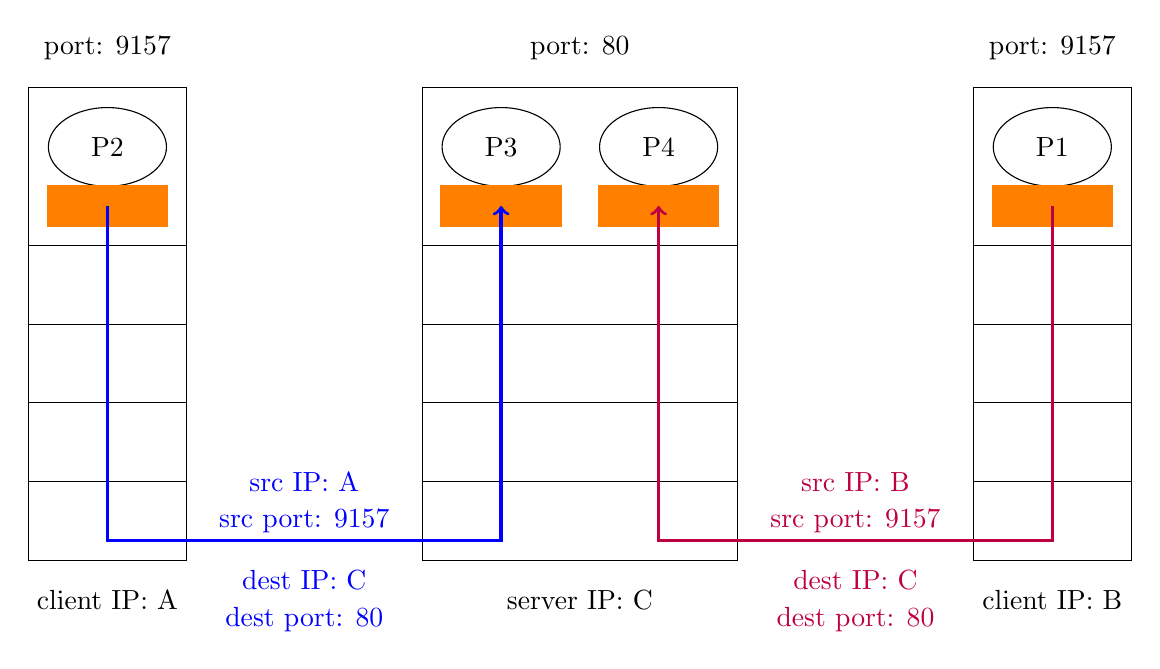
\begin{tikzpicture}
		\draw (1,6.5) node {port: 9157};
		\draw (0,0) rectangle (2,6);
		\draw (0,1) -- (2,1);
		\draw (0,2) -- (2,2);
		\draw (0,3) -- (2,3);
		\draw (0,4) -- (2,4);
		\draw (1,-0.5) node {client IP: A};
		\draw (1,5.25) ellipse (0.75 and 0.5);
		\draw (1,5.25) node {P2};
		\draw[orange, very thick, fill] (0.25,4.25) rectangle (1.75,4.75);

		\draw (7,6.5) node {port: 80};
		\draw (5,0) rectangle (9,6);
		\draw (5,1) -- (9,1);
		\draw (5,2) -- (9,2);
		\draw (5,3) -- (9,3);
		\draw (5,4) -- (9,4);
		\draw (7,-0.5) node {server IP: C};
		\draw (6,5.25) ellipse (0.75 and 0.5);
		\draw (6,5.25) node {P3};
		\draw[orange, very thick, fill] (5.25,4.25) rectangle (6.75,4.75);
		\draw (8,5.25) ellipse (0.75 and 0.5);
		\draw (8,5.25) node {P4};
		\draw[orange, very thick, fill] (7.25,4.25) rectangle (8.75,4.75);

		\draw (13,6.5) node {port: 9157};
		\draw (12,0) rectangle (14,6);
		\draw (12,1) -- (14,1);
		\draw (12,2) -- (14,2);
		\draw (12,3) -- (14,3);
		\draw (12,4) -- (14,4);
		\draw (13,-0.5) node {client IP: B};
		\draw (13,5.25) ellipse (0.75 and 0.5);
		\draw (13,5.25) node {P1};
		\draw[orange, very thick, fill] (12.25,4.25) rectangle (13.75,4.75);

		\draw[->, very thick, blue] (1,4.5) -- (1,0.25) -- (6,0.25) -- (6,4.5);
		\draw[blue] (3.5,1) node {src IP: A};
		\draw[blue] (3.5,0.5) node {src port: 9157};
		\draw[blue] (3.5,-0.25) node {dest IP: C};
		\draw[blue] (3.5,-0.75) node {dest port: 80};

		\draw[->, very thick, purple] (13,4.5) -- (13,0.25) -- (8,0.25) -- (8,4.5);
		\draw[purple] (10.5,1) node {src IP: B};
		\draw[purple] (10.5,0.5) node {src port: 9157};
		\draw[purple] (10.5,-0.25) node {dest IP: C};
		\draw[purple] (10.5,-0.75) node {dest port: 80};
	\end{tikzpicture}
	\caption{面向连接的多路复用与多路分解}
\end{figure}

\newpage

\section{无连接运输UDP}

\subsection{无连接运输UDP}

使用UDP时,在发送报文段之前,发送方和接收方的运输层实体之间没有握手。正因为如此,UDP被称为是无连接的。\\

UDP尽最大努力将数据包交付到目的主机,但不保证可靠性和顺序,也不保证带宽及延迟要求。UDP相较于TCP的优势包括无需连接建立、无连接状态、分组首部开销小。\\

\begin{table}[H]
	\centering
	\begin{tabular}{|p{3cm}<{\centering}|p{3cm}<{\centering}|}
		\hline
		source port \# & dest port \#                    \\
		\hline
		length         & checksum                        \\
		\hline
		\multicolumn{2}{|c|}{application data (message)} \\
		\hline
	\end{tabular}
	\caption{UDP报文段结构}
\end{table}

UDP首部只有4个字段,每个字段由2个字节组成,通过端口号可以将应用数据交给运行在目的端系统中的相应进程。长度字段指示了UDP报文段中的字节数(包括首部)。检验和可以用来检查该报文段中是否出现了差错。\\

\subsection{校验和(Checksum)}

当UDP报文段从源到达目的地的过程中,其中的bit有可能会受到噪声干扰或在路由器中存储而发生改变。UDP检验和提供了差错检测的功能。发送方对UDP报文段中所有内容都当作16位整数进行求和,在求和时遇到的溢出都需要被回卷(wraparound),再对和进行求反,得到的结果被放在UDP报文段中的检验和字段。\\

例如两个16位的整数相加:

\begin{table}[H]
	\centering
	\begin{tabular}{cD{.}{.}{3}}
		  & 1110011001100110  \\
		+ & 1101010101010101  \\
		\hline
		= & 11011101110111011
	\end{tabular}
\end{table}

将溢出位进行回卷:

\begin{table}[H]
	\centering
	\begin{tabular}{cD{.}{.}{3}}
		  & 1011101110111011 \\
		+ & 1                 \\
		\hline
		= & 1011101110111100
	\end{tabular}
\end{table}

计算反码得到校验和0100010001000011。\\

接收方收到报文段后,将所有16位整数相加(包括检验和)。如果该分组中没有差错,则计算得到的和将是1111111111111111,否则说明分组中有差错。\\

当检验和错误的时候,该分组一定错误,将会被丢弃。但是当检验和没有错误时,并不能保证分组是完全正确的。虽然UDP提供差错检测,但它对差错恢复无能无力。

\newpage